\begin{titlepage}

\newgeometry{top=0mm,right=20mm,left=20mm,bottom=0mm}



	%--------------------  Entete de l'Ecole ----------------------%

	\begin{figure}[t]
		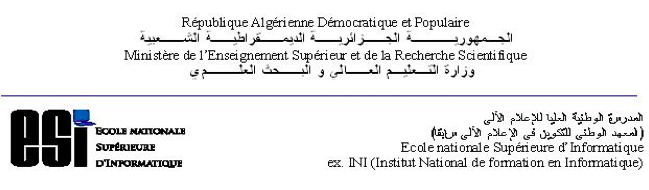
\includegraphics[scale=0.75]{./ressources/image/ESI.png}\\[0.6in]
	\end{figure}
	
	
	
	%--------------------------------------------------------------%
	\begin{center}
	
	%------------------------  Le sujet ---------------------------%
		\LARGE \textbf{ Mémoire}\\
		\Large{
			Pour Obtention du diplôme de Master En Informatique\\
			\textbf{Option : Système Informatique (SIQ)}
			%\textsc thèse D'Ingéniorat En Informatique sous le thème :
		}\\
		\huge {
		\rule{\linewidth}{.5pt}
			\textbf{
				Compression de Graphes par extraction de motifs et k2-trees : étude et implémentation
			} 
			\rule{\linewidth}{.5pt}
		}\\[0.4in]
		\Large
	%--------------------------------------------------------------%	
	
	%-------------------------  Mon nom ---------------------------%
	\textbf{Réaliser par:}\\
	\begin{multicols}{2}
			\Large 	Mlle. Hafsa Bousbiat\\
			\large eh\_bousbiat@esi.dz\\
			ESI\\
		\columnbreak
 			\Large Mlle. Sana Ihadadene\\
			\large es\_ihadadene@esi.dz\\
			ESI \\
		
	\end{multicols} 
	
	\vskip 0.13in
	%--------------------------------------------------------------%	

	%-----------------------  Encadreures -------------------------%
	 \textbf{Encadreurs:}\\
	 
	 \begin{multicols}{3}
			\Large 	Dr. Karima Amrouche\\
			\large k\_amrouche@esi.dz\\
			ESI\\
		\columnbreak
 			\Large Dr. Hamida Seba\\
			\large hamida.seba@univ-lyon1.fr\\
			Université de Lyon \\
		\columnbreak
 			\Large Dr. Mohammed Haddad\\
			\large mail\\
			Université de Lyon \\
	\end{multicols}
	
	%--------------------------------------------------------------%	
	
	\small
	\vskip 0.5in
	Octobre 2018 \\
	Année Universitaire: 2018-2019\\
	
	\end{center}		
\restoregeometry
\end{titlepage}